%==============================================================================
\section{Simulation Input}
\label{sec:sim_input}
%==============================================================================

In this section, the actual values of the inputs required by \papa as described
in Sec.~\ref{sec:papa_code} will be presented as they were used to generate the
results reported in Sec.~\ref{sec:results_baseline}. The detector-related
inputs were extracted from the official PINGU Monte Carlo datasets for geometry
V36\footnote{These are the PINGU Monte Carlo runs 390 for \nue and \nuebar, 389
for \numu and \numubar, and 390 for \nutau and \nutaubar.}.

\subsection{Atmospheric Neutrino Flux}
\label{sec:input_flux}

\begin{figure}[htbp]
 \centering
 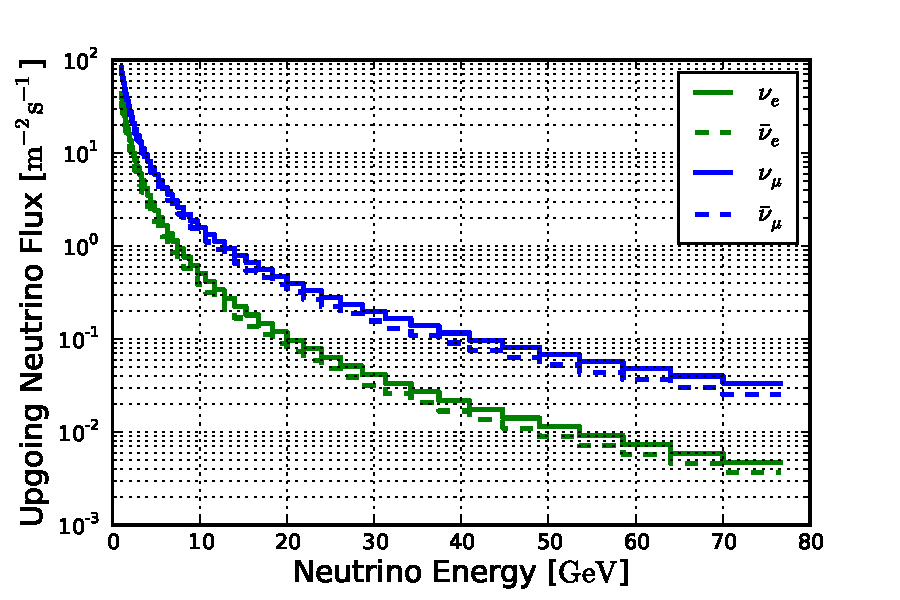
\includegraphics[width=0.7\linewidth]{summed_flux}
 \caption{The atmospheric neutrino flux at the South Pole integrated over all
          upgoing (\coszen in $[-1,0]$) directions. Based on the
          azimuth-averaged neutrino flux tables from \cite{HondaSP}.}
\label{fig:summed_flux}
\end{figure}

As already mentioned, the incoming atmospheric neutrino flux without
oscillations is calculated from the 2014 re-calculation of the flux tables
published by Honda et al.\ \cite{Honda, HondaSP}. A plot of the flux in the
energy range covered by the PINGU simulation (1\,--\,80\,GeV) is shown in
Fig.~\ref{fig:summed_flux}. The flux has been integrated over all upgoing
(\coszen in $[-1,0]$) directions, as downgoing neutrinos arriving from above
the detector do not pass through a significant amount of matter and hence do
not bear any information on the neutrino mass hierarchy.

\subsection{Oscillation Probabilities}
\label{sec:input_osc}

The neutrino oscillation probabilities have been calculated using the
AtmoWeights code for the PREM Earth density profile as described in
Sec.~\ref{sec:PINGUosc}. The fiducial values of the mixing parameters used for
the calculation follow the global fit of Fogli et al.\ \cite{Fogli}, listed in
Tab.~\ref{tab:fiducial_osc}. Example plots of the probabilities demonstrating
the characteristic signature of the mass hierarchy are shown in high resolution
in that section as well, the full set of all possible oscillation channels can
be found in App.~\ref{app:oscillation}. The binning of those plots is the same
as used for the actual analysis, which is 79 logarithmic bins in energy between
1\,GeV and 80\,GeV and 20 equally sized bins between -1 and 0 in \coszen.

\subsection{Effective Areas}
\label{sec:input_aeff}

\begin{figure}[htbp]
 \centering
 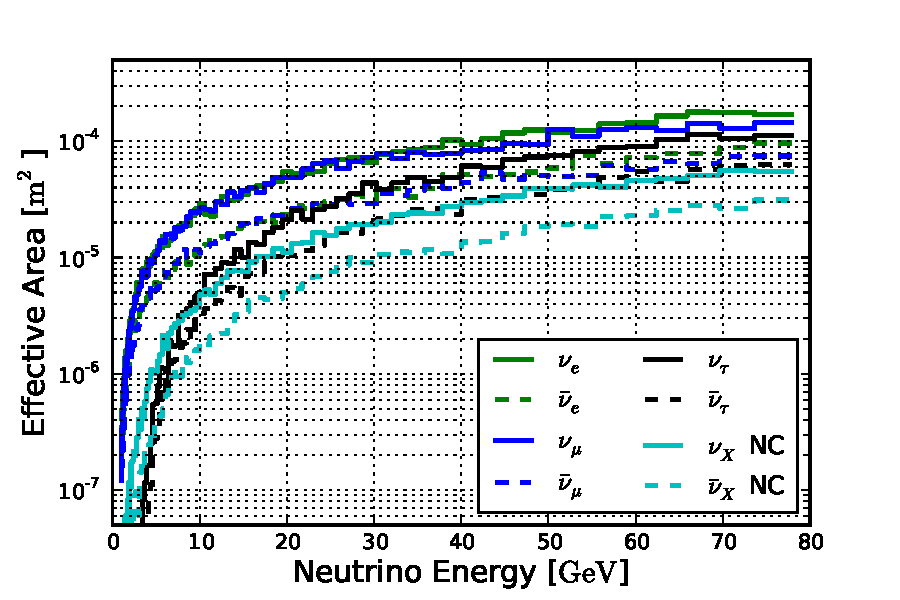
\includegraphics[width=0.495\linewidth]{aeff_energy}
 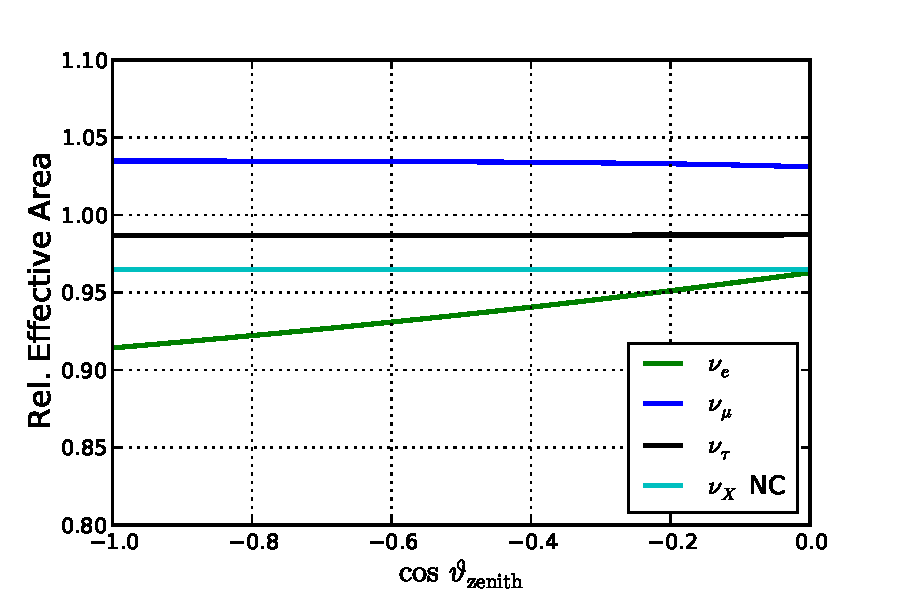
\includegraphics[width=0.495\linewidth]{aeff_coszen}
 \caption{Effective areas for all relevant neutrino interactions. Shown are
  energy (left)  and zenith (right) dependence.}
\label{fig:aeffs}
\end{figure}

The effective areas are extracted from PINGU Monte Carlo datasets via the
OneWeight quantity multiplied by $4\pi$, which is equivalent to a per-event
effective area \cite{OneWeight}. The zenith dependence of the effective area is
modelled by an analytic fit to the MC data, assuming that energy and zenith
dependence can be handled separately. A plot of the effective areas and their
zenith dependence is shown in Fig.~\ref{fig:aeffs}.

\subsection{Reconstruction Resolutions}
\label{sec:input_reco}

As already mentioned, the event reconstruction for the baseline model will be
simulated by 


% \begin{figure}
%  \centering
%  \includegraphics[width=0.495\linewidth]{figures/MultiNest_EnergyResolution.pdf}
%  \includegraphics[width=0.495\linewidth]{figures/MultiNest_ZenithResolution.pdf}
%  \caption{Median resolutions of the \textsf{MultiNest} algorithm for
%   $\nu_e/\bar\nu_e$ and $\nu_\mu/\bar\nu_\mu$ CC events.
%   \emph{Left:} Relative energy resolution.
%   \emph{Right:} Zenith angle resolution}
%  \label{fig:MultiNest}
% \end{figure}


The input for the reconstruction resolutions, whether supplied as
parametrisations or tables, is obtained from the
\textsf{MultiNest}\footnote{Developed by J.\,P.\ A.\,M.\ de Andr\'{e},
M.\ Dunkman, and F.\ Huang (Penn State)} reconstruction algorithm. This 8D
hybrid likelihood minimization fits for the hadronic interaction vertex plus an
outgoing muon. Median resolutions in energy and zenith angle are shown in
Fig.~\ref{fig:MultiNest}.

\subsection{Particle Flavour Identification}
\label{sec:input_pid}

\begin{figure}[htbp]
 \centering
 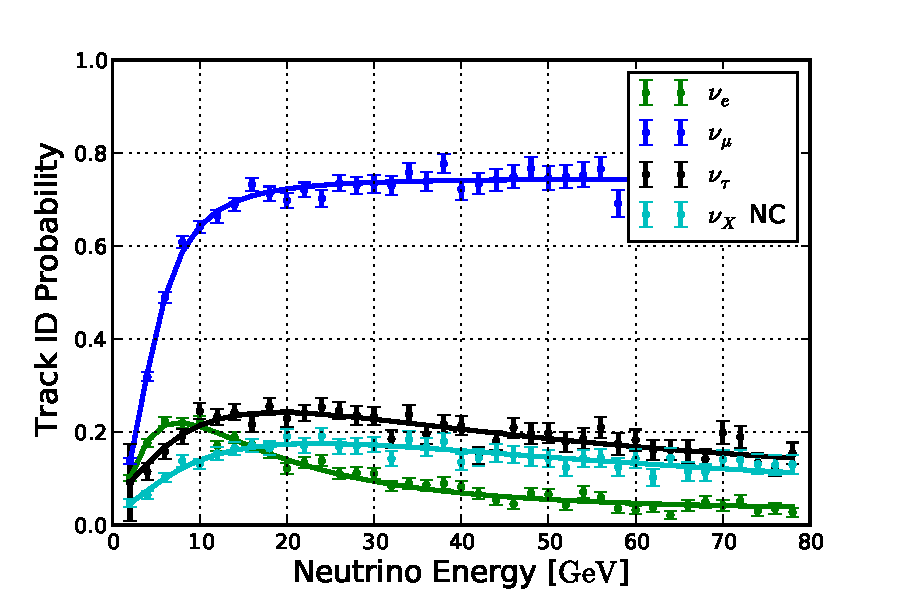
\includegraphics[width=0.7\textwidth]{PID}
 \caption{Track identification probability as function of energy in all four
  interaction channels. The straight lines show fits to the data.}
 \label{fig:PID}
\end{figure}

The classification of the neutrino events into track-like and cascade-like
events is according to their final score in the boosted decision tree described
in Sec.~\ref{sec:cuts_PID}. In the baseline detector settings, the decision is
of binary nature, meaning that the probability to classify a given event as
cascade is one minus the probability to classify it as a track.

Data points for the track identification probabilities in all channels as a
function of the neutrino energy have been provided by \cite{JP_PID}. These data
were fitted with analytic functions, the fits are shown together with the data
points in Fig.~\ref{fig:PID}. The functions definitions themselves are listed
in App.~\ref{app:pid}.